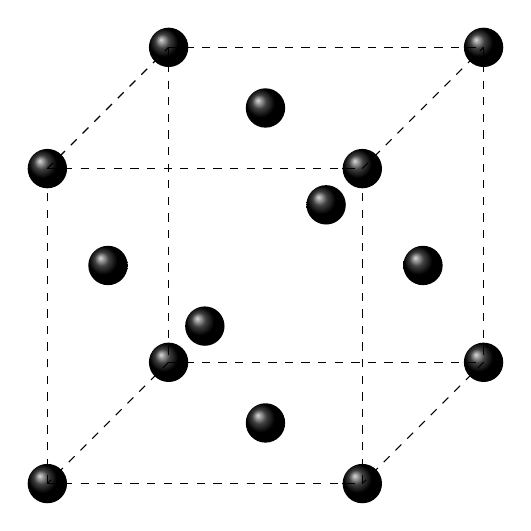
\begin{tikzpicture}
    %points on cube
    \coordinate (A) at (0,0,0);
    \coordinate (B) at (0,0,4);
    \coordinate (D) at (0,4,0);
    \coordinate (C) at (0,4,4);
    \coordinate (E) at (4,0,0);
    \coordinate (F) at (4,0,4);
    \coordinate (H) at (4,4,0);
    \coordinate (G) at (4,4,4);

    %center of faces
    \coordinate (I) at (0,2,2); %center of face ABCD
    \coordinate (J) at (4,2,2); %center of face EFGH
    \coordinate (K) at (2,4,2); %center of face DCGH
    \coordinate (L) at (2,0,2); %center of face ABFE
    \coordinate (M) at (2,2,4); %center of face CBGF
    \coordinate (N) at (2,2,0); %center of face DAEH

    %place non-atom cube corners
    \shade [ball color= black] (A) circle (0.25cm);
    \shade [ball color= black] (C) circle (0.25cm);
    \shade [ball color= black] (F) circle (0.25cm);
    \shade [ball color= black] (H) circle (0.25cm);
    \shade [ball color= black] (B) circle (0.25cm);
    \shade [ball color= black] (D) circle (0.25cm);
    \shade [ball color= black] (E) circle (0.25cm);
    \shade [ball color= black] (G) circle (0.25cm);

    %draw the center of each face
    \shade [ball color= black] (I) circle (0.25cm);
    \shade [ball color= black] (J) circle (0.25cm);
    \shade [ball color= black] (K) circle (0.25cm);
    \shade [ball color= black] (L) circle (0.25cm);
    \shade [ball color= black] (M) circle (0.25cm);
    \shade [ball color= black] (N) circle (0.25cm);

    %draw cube
    \draw [dashed] (A) -- (B);
    \draw [dashed] (B) -- (C);
    \draw [dashed] (C) -- (D);
    \draw [dashed] (D) -- (A);
    \draw [dashed] (E) -- (F);
    \draw [dashed] (F) -- (G);
    \draw [dashed] (G) -- (H);
    \draw [dashed] (H) -- (E);
    \draw [dashed] (A) -- (E);
    \draw [dashed] (B) -- (F);
    \draw [dashed] (C) -- (G);
    \draw [dashed] (D) -- (H);
\end{tikzpicture}
